%! Author = Len Washington III
%! Date = 9/12/2023

% Preamble
\documentclass[28]{cs430lecture}

% Packages

% Document
\begin{document}

%<*Lecture-Activity-28>
\maketitle
\openingquestions
\begin{itemize}
	\item We saw the \hyperref[sec:shortest-path-algorithm-bellman-ford]{Bellman-Ford} algorithm found the
	shortest path from a source to all other vertices by ``brute force''
	every edge in the graph in a fixed order $|V|-1$ times.
	Why did it need to do this $|V|-1$ times?
	And with this in mind, could we improve on the Bellman-Ford for certain graphs?
	\begin{answer}
		At least relax edges leaving from source first.
		Possible that the shortest path $u\leadsto v$ goes through every other vertex $|V|-1$ edges might be relaxed in opposite order.
	\end{answer}
\end{itemize}

\section{DAG Shortest Path Algorithm}\label{sec:dag-shortest-path-algorithm}
By relaxing the edges of a weighed DAG (directed acyclic graph) $G=(V,E)$ in topological sort order of its vertices, we can compute shortest paths from a single source.
Shortest paths are always defined in a DAG, since even if there are negative-weight edges, no negative weight cycles can exist.
\begin{algorithm}[H]
	\caption{DAG Shortest Path\begin{answer}$O(V^{2})$\end{answer}}\label{alg:dag-shortest-path}
	\begin{algorithmic}[1]
	\Function{DAG-Shortest-Path}{$G$, $w$, $s$}
		\State \hyperref[alg:topological-sort]{topologically sort} the vertices of $G$
		\State \Call{\hyperref[alg:init-single-source]{Init-Single-Source}}{$G$, $s$}
		\ForAll{vertex $u$, taken in topologically sorted order}
			\ForAll{vertex $v\in Adj[u]$}
				\State \Call{\hyperref[alg:relax]{Relax}}{$u$, $v$, $w$}
			\EndFor
		\EndFor
	\EndFunction
	\end{algorithmic}
\end{algorithm}

\begin{enumerate}
    \item Here is the topological sort on a DAG\@.
	Find the shortest path from $s$ to every other vertex.
	\item What is the runtime for DAG Shortest Path?
	\begin{answer}$O(|V|+|E|)\Rightarrow O(|V|+|V|^{2})\Rightarrow O(|V|^{2})$\end{answer}
	\item Discuss why DAG Shortest Path is correct.
	\begin{answer}
		Given a source, you relax an edge, the incremental improvement on source path estimate.
	\end{answer}
	\item If we restrict the graph to having no negative edges, given a source $s$, what is the shortest path from $s$ to one of its adjacent vertices?
	\begin{answer}
		\begin{figure}[H]
			\centering
			\begin{tikzpicture}[scale=1.5]
				\begin{scope}\globalnodeset
					\node[label=left:Source] (s) at (0,0) {$0$};
					\node (t) at (2,2) {$\infty$};
					\node (x) at (2,0) {$\infty$};
					\node (z) at (2,-2) {$\infty$};
				\end{scope}
				\begin{scope}\globalpathset
					\path [->] (s) edge node {$3$} (t);
					\path [->] (s) edge node {$4$} (x);
					\path [->] (s) edge node {$5$} (z);
				\end{scope}
			\end{tikzpicture}
			\caption{$3$ is done, because there is no negative path that could go from one of the other nodes to it.
			$4$ and $5$ are not done because there could be paths with values that could create a better estimate like $\frac{1}{2}$ and $1$ respectively.}
			\label{fig:restricted}
		\end{figure}
	\end{answer}
\end{enumerate}

\section{Dijkstra's Shortest Path Algorithm}\label{sec:dijkstra's-shortest-path-algorithm}
\begin{itemize}
	\item No negative-weight \emph{edges}.
	\item Essentially a weighted version of breadth-first search.
	\begin{itemize}
		\item Instead of a FIFO queue, uses a priority queue.
		\item Keys are shortest-path weight estimates ($d[v]$).
	\end{itemize}
	\item Have two sets of vertices:
	\begin{itemize}
		\item $S=$ vertices whose final shortest-path weights are determined,
		\item $Q=$ priority queue = $V-s$.
	\end{itemize}
	\item Dijkstra's algorithm can be viewed as greedy, since it always chooses the ``lightest'' (``closest'') vertex in $V-S$ to add to $S$.
\end{itemize}

\begin{algorithm}[H]
	\caption{Dijkstra}\label{alg:dijkstra}
	\begin{algorithmic}[1]
	\Function{Dijkstra}{$V$, $E$, $w$, $s$}
		\State \Call{\hyperref[alg:init-single-source]{Init-Single-Source}}{$V$, $s$}
		\State $S\gets\emptyset$
		\State $Q\gets V$												\Comment{i.e., insert all vertices into $Q$ by $d$ values}
		\While{$Q$ is not empty}
			\State $u\gets\Call{\hyperref[subsec:Extract-Min]{Extract-Min}}{Q}$
			\State $S\gets S \cup \{ u \}$
			\ForAll{vertex $v\in Adj[u]$}
				\State \Call{\hyperref[alg:relax]{Relax}}{$u$, $v$, $w$}\Comment{Possibly updates a short path estimate $d$ value and moves the vertex forward in the queue}
			\EndFor
		\EndWhile
	\EndFunction
	\end{algorithmic}
\end{algorithm}

\begin{enumerate}[start=5]
    \item Here is a graph with non negative edges.
	Find the shortest path from $s$ to every other vertex using Dijkstra's algorithm.
	\begin{figure}[H]
		\centering
		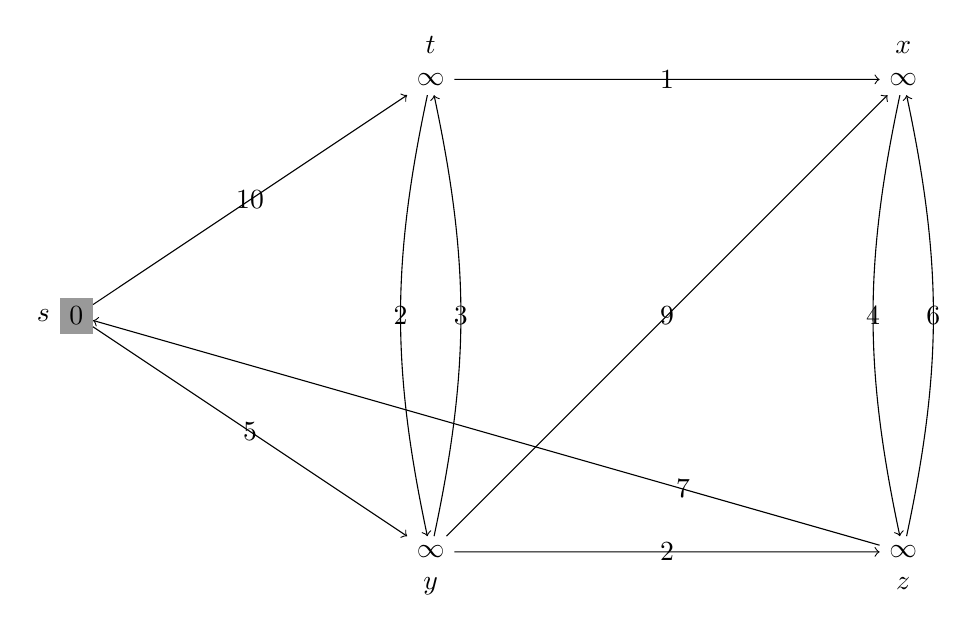
\begin{tikzpicture}[scale=1.5]
			\begin{scope}\globalnodeset
				\node[label=left:$s$,fill=gray!80!white] (s) at (-1,0) {$0$};
				\node[label=above:$t$] (t) at (2,2) {$\infty$};
				\node[label=above:$x$] (x) at (6,2) {$\infty$};
				\node[label=below:$y$] (y) at (2,-2) {$\infty$};
				\node[label=below:$z$] (z) at (6,-2) {$\infty$};
			\end{scope}
			\begin{scope}\globalpathset
				\path [->] (s) edge node {$5$} (y);
				\path [->] (s) edge node {$10$} (t);

				\path [->] (t) edge node {$1$} (x);

				\path [->] (y) edge node {$2$} (z);
				\path [->] (y) edge node {$9$} (x);

				\path [->] (z) edge[near start] node {$7$} (s);

				\path [->] (t) edge[bend right=12] node {$2$} (y);
				\path [->] (y) edge[bend right=12] node {$3$} (t);

				\path [->] (x) edge[bend right=12] node {$4$} (z);
				\path [->] (z) edge[bend right=12] node {$6$} (x);
			\end{scope}
		\end{tikzpicture}
		\label{fig:dijkstra-algorithm-example}
	\end{figure}
	\item What is the runtime for Dijkstra's algorithm?
	\item Prove the greedy choice in Dijkstra's algorithm (pick the vertex with the smallest shortest path estimate, not including the vertices we are done with) leads to an optimal solution.
\end{enumerate}

Dijkstra's Algorithms\\
\url{https://www.youtube.com/watch?v=wtdtkJgcYUM}\\
\url{https://www.cs.usfca.edu/~galles/visualization/Dijkstra.html}
%</Lecture-Activity-28>

\end{document}